\chapter{Neutral Diversity and Population Structure.}
%% this section was moved from the coalescent chapter
We've considered alleles drawn from a randomly-mating population, and divergence among alleles drawn from two distantly-related populations.
We'll now turn to consider divergence among more closely related populations. In thinking about the coalescent  within populations we made the assumption that any pair of lineages is equally likely to coalesce with each
other. However, when there is population structure this assumption is violated. \\

We have previously written the measure of population structure
$\fst$ as
\begin{equation}
\fst = \frac{H_T-H_S}{H_T}
\end{equation}
where $H_S$ is the probability that two alleles sampled at random from a
subpopulation differ, and $H_T$ is the probability that two alleles
sampled at random from the total population differ.

\paragraph{A simple population split model}
Imagine a population of constant size of $N_e$ diploid individuals that
$T$ generations in the past split into two daughter populations (sub-populations)
each of size $N_e$ individuals, which do not subsequently exchange
migrants. In the current day we sample an equal number of alleles
from both subpopulations.

\begin{figure}
\begin{center}
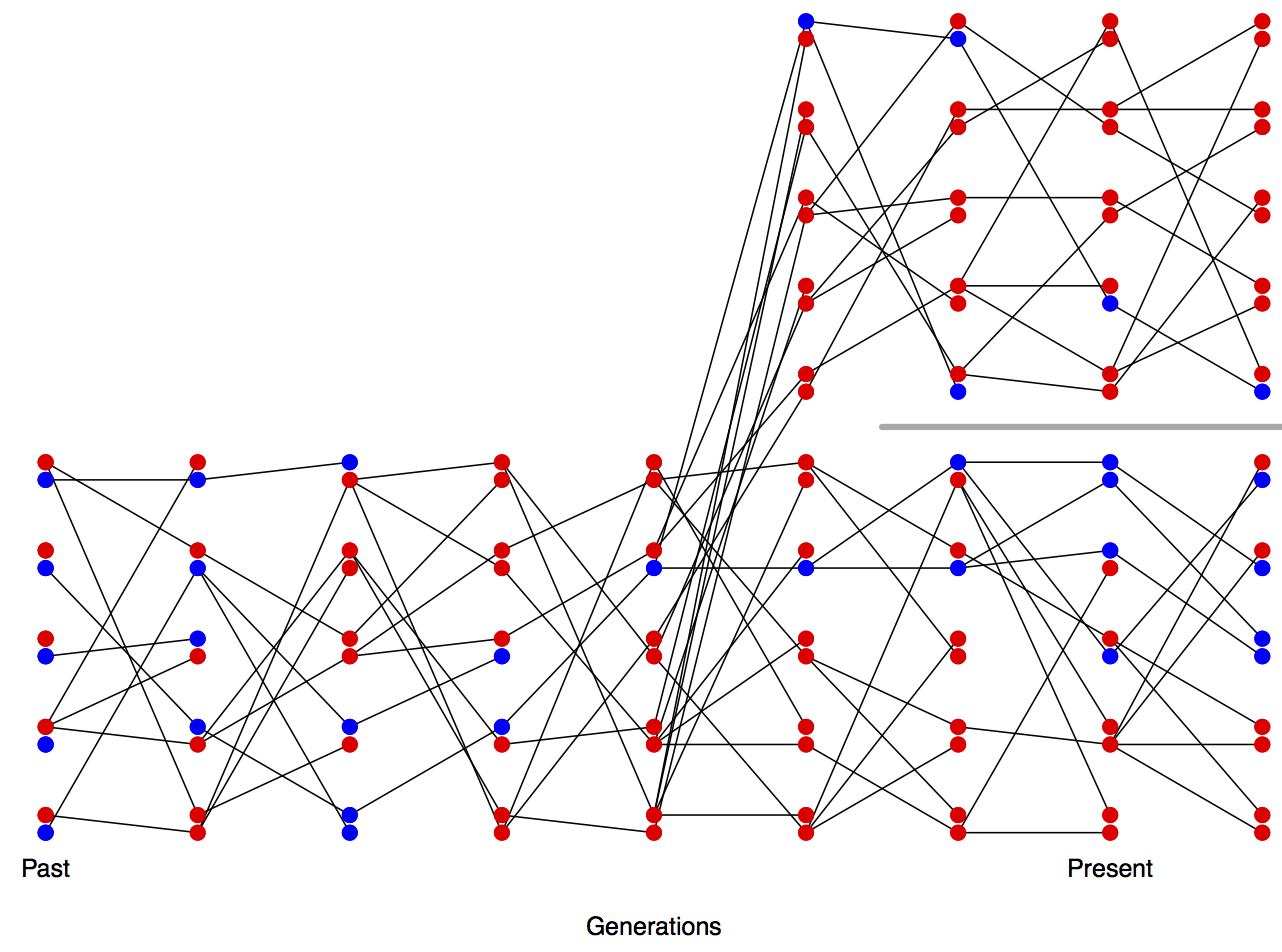
\includegraphics[width= 0.8 \textwidth]{figures/drift_split.png}
\end{center}
\caption{Change in allele frequencies following a population split. \gitcode{https://github.com/cooplab/popgen-notes/blob/master/Rcode/Loss_of_heterozyg_varying_pop.R}} \label{fig:drift_split}
\end{figure}

Consider a pair of alleles sampled within one of our
sub-populations and think about their per site heterozygosity.
These alleles have experienced a population of size $N_e$
and so the probability that they differ is $H_S \approx 4N_e \mu$ (assuming that $N_e \mu \ll 1$, using our equation  \ref{eqn:hetero} for heterozygosity within a population ).

%Consider a pair of alleles sampled within one of our
%sub-populations, they have experienced a population of size $N_e$
%and so the probability that they differ is $H_S = \theta/(1+\theta)$
%(where $\theta=4N_e\mu$).


The heterozygosity in our total population is a little more tricky to
calculate. Assuming that we equally sample both sub-populations, when we draw two alleles from our total
sample, $50\%$ of the time they are drawn from the same
subpopulation and $50\%$ of the time they are drawn from different
subpopulations. Therefore, our total heterozygosity is given by
\begin{equation}
H_T = \half H_S + \half H_B
\end{equation}
where $H_B$ is the probability that a pair of alleles drawn from our
two different sub-populations differ from each other. A pair of
alleles from different sub-populations cannot find a common ancestor with each other for at least $T$
generations into the past as they are in distinct populations (not
connected by migration). Once our alleles find themselves back in the combined ancestral
population it takes them on average $2N$ generations to coalesce. So the total opportunity for mutation between our pair of alleles sampled from different populations is $2 (T + 2N )$ generations of meioses, such that the probability that our pairs of alleles is different is
\begin{equation}
H_B \approx 2\mu ( T + 2 N) %\left( 1-(1-\mu)^{2T} \right) + (1-\mu)^{2T}
  %\frac{\theta}{\theta+1}
\end{equation}


%The probability that one or other of them
%mutates in this time is $1-(1-\mu)^{2T}$. With probability
%$(1-\mu)^{2T} $ neither of our alleles mutate in the $T$ generations
%back in time before they find themselves back in the combined ancestral
%population. Conditional on failing to mutate before the combined ancestral
%population, the probability that they do manage to mutate before
%coalescing in that population of size $N_e$ is
%$\theta/(\theta+1)$. Putting these components together
%\begin{equation}
%H_B = \left( 1-(1-\mu)^{2T} \right) + (1-\mu)^{2T}
 % \frac{\theta}{\theta+1}
%\end{equation}
We can plug this into our expression for $H_T$, and then that in turn
into $\fst$. Doing so we find that
\begin{equation}
\fst \approx \frac{ \mu T}{\mu T +  4N_e\mu }  = \frac{ T}{ T +  4N_e }
\end{equation}
Note that $\mu$ cancels out of this equation. In this simple toy model, $\fst$
is increasing because the amount of between-population diversity
increases with the divergence time of the two populations (initially
linearly with $T$). $\fst$ grows at a rate
give by $\nicefrac{T}{(4N_e)}$ so that differentiation will be higher
between populations separated by long divergence times or with small
effective population sizes.

\begin{marginfigure}
\begin{center}
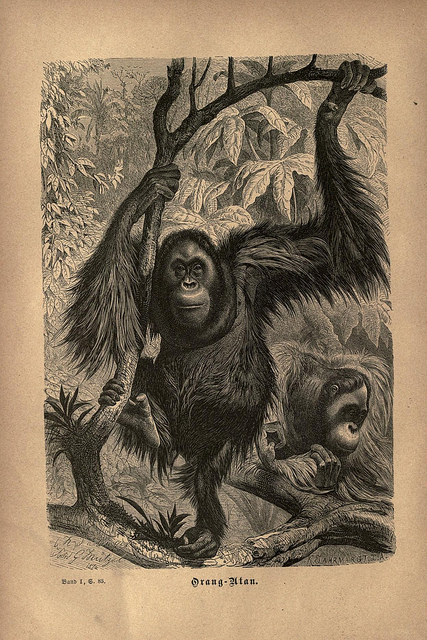
\includegraphics[width= 0.8 \textwidth]{illustration_images/Genetic_drift/Orang/7971889392_d32b45668b_z.jpg}
\end{center}
\caption{Orangutan ({\it Pongo}). \BHLNC{Brehms thierleben, allgemeine kunde des thierreichs. Brehm, A. E.}{https://www.biodiversitylibrary.org/page/1008013\#page/114/mode/1up}{MBLWHOI Library}} \label{fig:Orang}
\end{marginfigure}


\begin{question}  %Pongo abelii (Sumatran) and Pongo pygmaeus
  The genome-wide $F_{ST}$ between Bornean and Sumatran orangutan species samples  ({\it Pongo pygmaeus} and {\it Pongo abelii}) is $\approx 0.37$ \citep{locke2011}, representing a deep population split between the species (potentially with little subsequent gene flow). Within the populations the genome-wide average Watterson's $\theta$ is $\theta_W=1.4$kb$^{-1}$, estimated from the number of segregating sites. Assume a generation time of 20 years, and a mutation rate of $2 \times 10^{-8}$ per base per generation. How far in the past did the two populations diverge?
\end{question}
%o understand this better we can make a simple
%approximation based on our mutation rate being very low, such that
%$N_e \mu \ll 1$ so $H_S \approx
%4N_e\mu$, and that $\mu \ll 1$ and $\mu T \ll 1$. Assuming this, then
%\begin{equation}
%H_B \approx 2 \mu T + 4N_e\mu.
%\end{equation}



%\begin{question}
%The gorilla lineage split from the human-chimp lineage $\sim$7 million years ago. Let’s assume that this speciation event occurred instantaneously in allopatry with no subsequent gene flow. \\
%{\bf A)}	What is the probability of that gorilla is not an outgroup to human and chimp at a single locus?\\
%{\bf B)}	It has been estimated that the gorilla lineage is not an outgroup at around ~30\% of autosomal loci. What effective population size would you need to assume to explain this observation? Is that only plausible explanation?\\
%{\bf C)}	The gorilla lineage is an outgroup for large portions of the X chromosome, what is a plausible explanation for this finding?
%\end{question}

\paragraph{A simple model of migration between an island and the mainland.}
We can also use the coalescent to think about patterns of
differentiation under a simple model of migration-drift
equilibrium. Let's consider a small island population that is relatively isolated
from a large mainland population, where both of these populations
are constant in size. We'll assume that the expected heterozygosity
for a pair of alleles sampled on the mainland is $H_M$.

Our island has a population size
$N_{I}$ that is very small compared to our mainland population.
Each generation some low fraction $m$ of our individuals on the
island have migrant parents from the mainland the generation
before. Our island may also send migrants back to the mainland, but
these are a drop in the ocean compared to the large population size on
the mainland and their effect can be ignored.


If we sample an allele on the island and trace its ancestral
lineage backward in time, each generation our ancestral allele has a low
probability $m$ of being descended from the mainland in the preceding
generation (if we go back far enough the allele eventually has to be
descended from an allele on the mainland). The probability that a pair of alleles sampled on the
island are descended from a shared recent common ancestral allele on the island is the
probability that our pair of alleles coalesces before either lineage
migrates. For example, the probability that our pair of alleles
coalesces $t+1$ generations back on the island is
\begin{equation}
\frac{1}{2N_I}(1-m)^{2(t+1)} \left(1-\frac{1}{2N_I} \right)^{t} \approx
\frac{1}{2N_I} \exp\left( -t\left (\frac{1}{2N_I} + 2m\right) \right),
\end{equation}
%JRI: this is a long scary-looking equation. i think it's pretty straightforward but even I was momentarily surprised by it. i think many readers will see it and tune out and not try to work through it. i suggest you keep it but spend a few sentences working through it (1-m) not migrating times prob. of coalesceing t gens, etc.
with the approximation following from assuming that $m \ll 1$ \& $\frac{1}{(2N_I)}
\ll 1$ (note that this is very similar to our derivation of
heterozygosity above). The probability that our alleles coalesce before either one
of them migrates off the island, irrespective of the time, is
\begin{equation}
\int_0^{\infty} \frac{1}{2N_I} \exp\left( -t\left (\frac{1}{2N_I} +
2m\right) \right) dt = \frac{\nicefrac{1}{(2N_I)}}{\nicefrac{1}{(2N_I)} +
    2m}.
\end{equation}

Let's assume that the mutation rate is very low such that it is very
unlikely that the pair of alleles mutate before they coalesce on the
island. Therefore, the only way that the alleles can be different from
each other is if one or other of them migrates to the mainland, which
happens with probability
\begin{equation}
  1 - \frac{\nicefrac{1}{(2N_I)}}{\nicefrac{1}{(2N_I)} + 2m}
\end{equation}
Conditional on one or other of our alleles migrating to the mainland, both of our alleles represent independent draws from the mainland and so differ from each other with probability $H_M$. Therefore, the level of
heterozygosity on the island is given by
\begin{equation}
  H_I = \left(1 - \frac{\nicefrac{1}{(2N_I)}}{\nicefrac{1}{(2N_I)} + 2m} \right)H_M
\end{equation}
So the reduction of heterozygosity on the island compared to the
mainland is
\begin{equation}
  F_{IM} = 1- \frac{H_I}{H_M} = \frac{\nicefrac{ 1}{(2N_I)}}{\nicefrac{1}{(2N_I)} + 2m} = \frac{ 1 }{1 + 4N_Im}.
\end{equation}
The level of inbreeding on the island compared to the mainland will be high if the migration rate is low and the effective population size of the island is low, as allele frequencies on the island are drifting and diversity on the island is not being replenished by migration. The
key parameter here is the number individuals on the island replaced by immigrants from the mainland each generation ($N_I m$).

We have framed this problem as being about the reduction in genetic diversity on the island compared to the mainland. However, if we consider collecting individuals on the island and mainland in proportion to their population
sizes, the total level of heterozygosity would be $H_T=H_M$, as samples from our mainland would greatly outnumber those from our island. Therefore, considering the island as our sub-population, we have derived another simple model of $F_{ST}$.

\begin{marginfigure}
\begin{center}
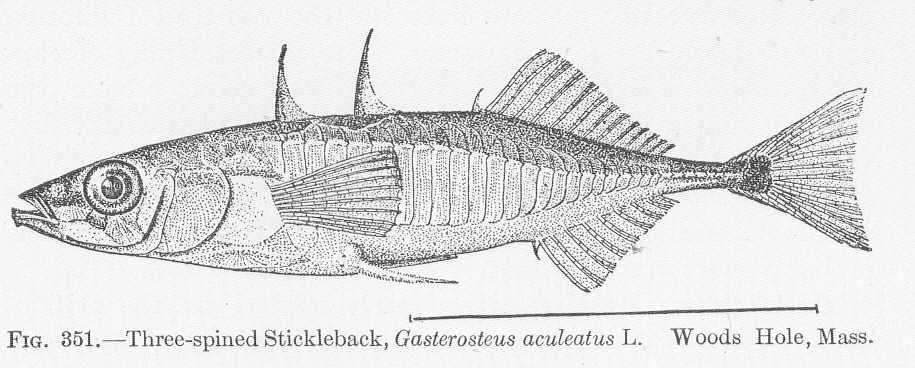
\includegraphics[width=\textwidth]{illustration_images/Genetic_drift/stickleback/threespine.jpg}
\end{center}
\caption{Three-spined stickleback ({\it Gasterosteus aculeatus}).
  \newline \noindent \tiny{Jordan, David Starr (1907) Fishes, New York City, NY: Henry Holt and Company. Image from  \href{https://commons.wikimedia.org/wiki/File:FMIB_51889_Three-spined_Stickleback,_Gasterosteus_aculeatus_L_Woods_Hole,_Mass.jpeg}{Wikimedia Commons} Public domain.}} \label{fig:stickle}
\end{marginfigure}

\begin{question}
You are investigating a small river population of sticklebacks, which receives infrequent migrants from a very large marine population. At a set of putatively neutral biallelic markers the freshwater population has frequencies:\\
0.2, 0.7, 0.8\\
at the same markers the marine population has frequencies:\\
0.4, 0.5 and 0.7.\\
 From studying patterns of heterozygosity at a large collection of markers, you have estimated the long term effective size of your freshwater population is 2000 individuals.\\
What is your estimate of the migration rate from the marine
populations into the river?
\end{question}

\paragraph{Incomplete Lineage Sorting}
Finally we turn to the interaction of 
Because it can take a long time for an polymorphism to drift up or down in frequency, multiple population splits may occur during the time an allele is still segregating. This can lead to incongruence between the overall population tree and the information about relationships present at
individual loci. In Figure \ref{fig:NoILS_poly} and \ref{fig:ILS_poly}
we show a simulation of three populations where the bottom population splits off from the other two first, followed by the subsequent splitting of the the top and the middle populations. We start both simulations with a newly
introduced red allele being polymorphic in the combined ancestral population. The most likely fate of this allele is that it is
quickly lost from the population, but sometimes the allele can drift up in frequency and be polymorphic when the populations split, as the allele in our two figures has done. If the allele is lost/fixed in the descendant populations before the next population split, our allele
configuration will agree with the population tree, as it does in
Figure  \ref{fig:NoILS_poly}, and so too the gene tree will agree with population tree (as shown in the left side of Figure \ref{fig:ILS_cartoon}).
However, if the allele persists as a polymorphism in the ancestral population until the top and the middle
populations split, then the allele could fix in one of these populations
and not the other. Such an event leads to a substitution pattern
that disagrees with the population tree, as in Figure \ref{fig:ILS_poly}.  If
we were to construct a phylogeny using the variation at this site we would see a disagreement between the gene tree and population tree. In Figure \ref{fig:ILS_poly} an allele
drawn from the top and the bottom populations are
necessarily more closely related to each other than either is to an allele drawn from population 2;
tracing our allelic lineages from the top and bottom populations back through time, they must coalesce with each other before we reach the point where the red mutation arose; in contrast, a lineage from the middle population cannot have coalesced with either other lineage until past the time the red mutation arose. An example of this `incomplete lineage sorting' in terms of the underlying tree is shown on the right side of Figure \ref{fig:ILS_cartoon}.


\begin{figure}
\begin{center}
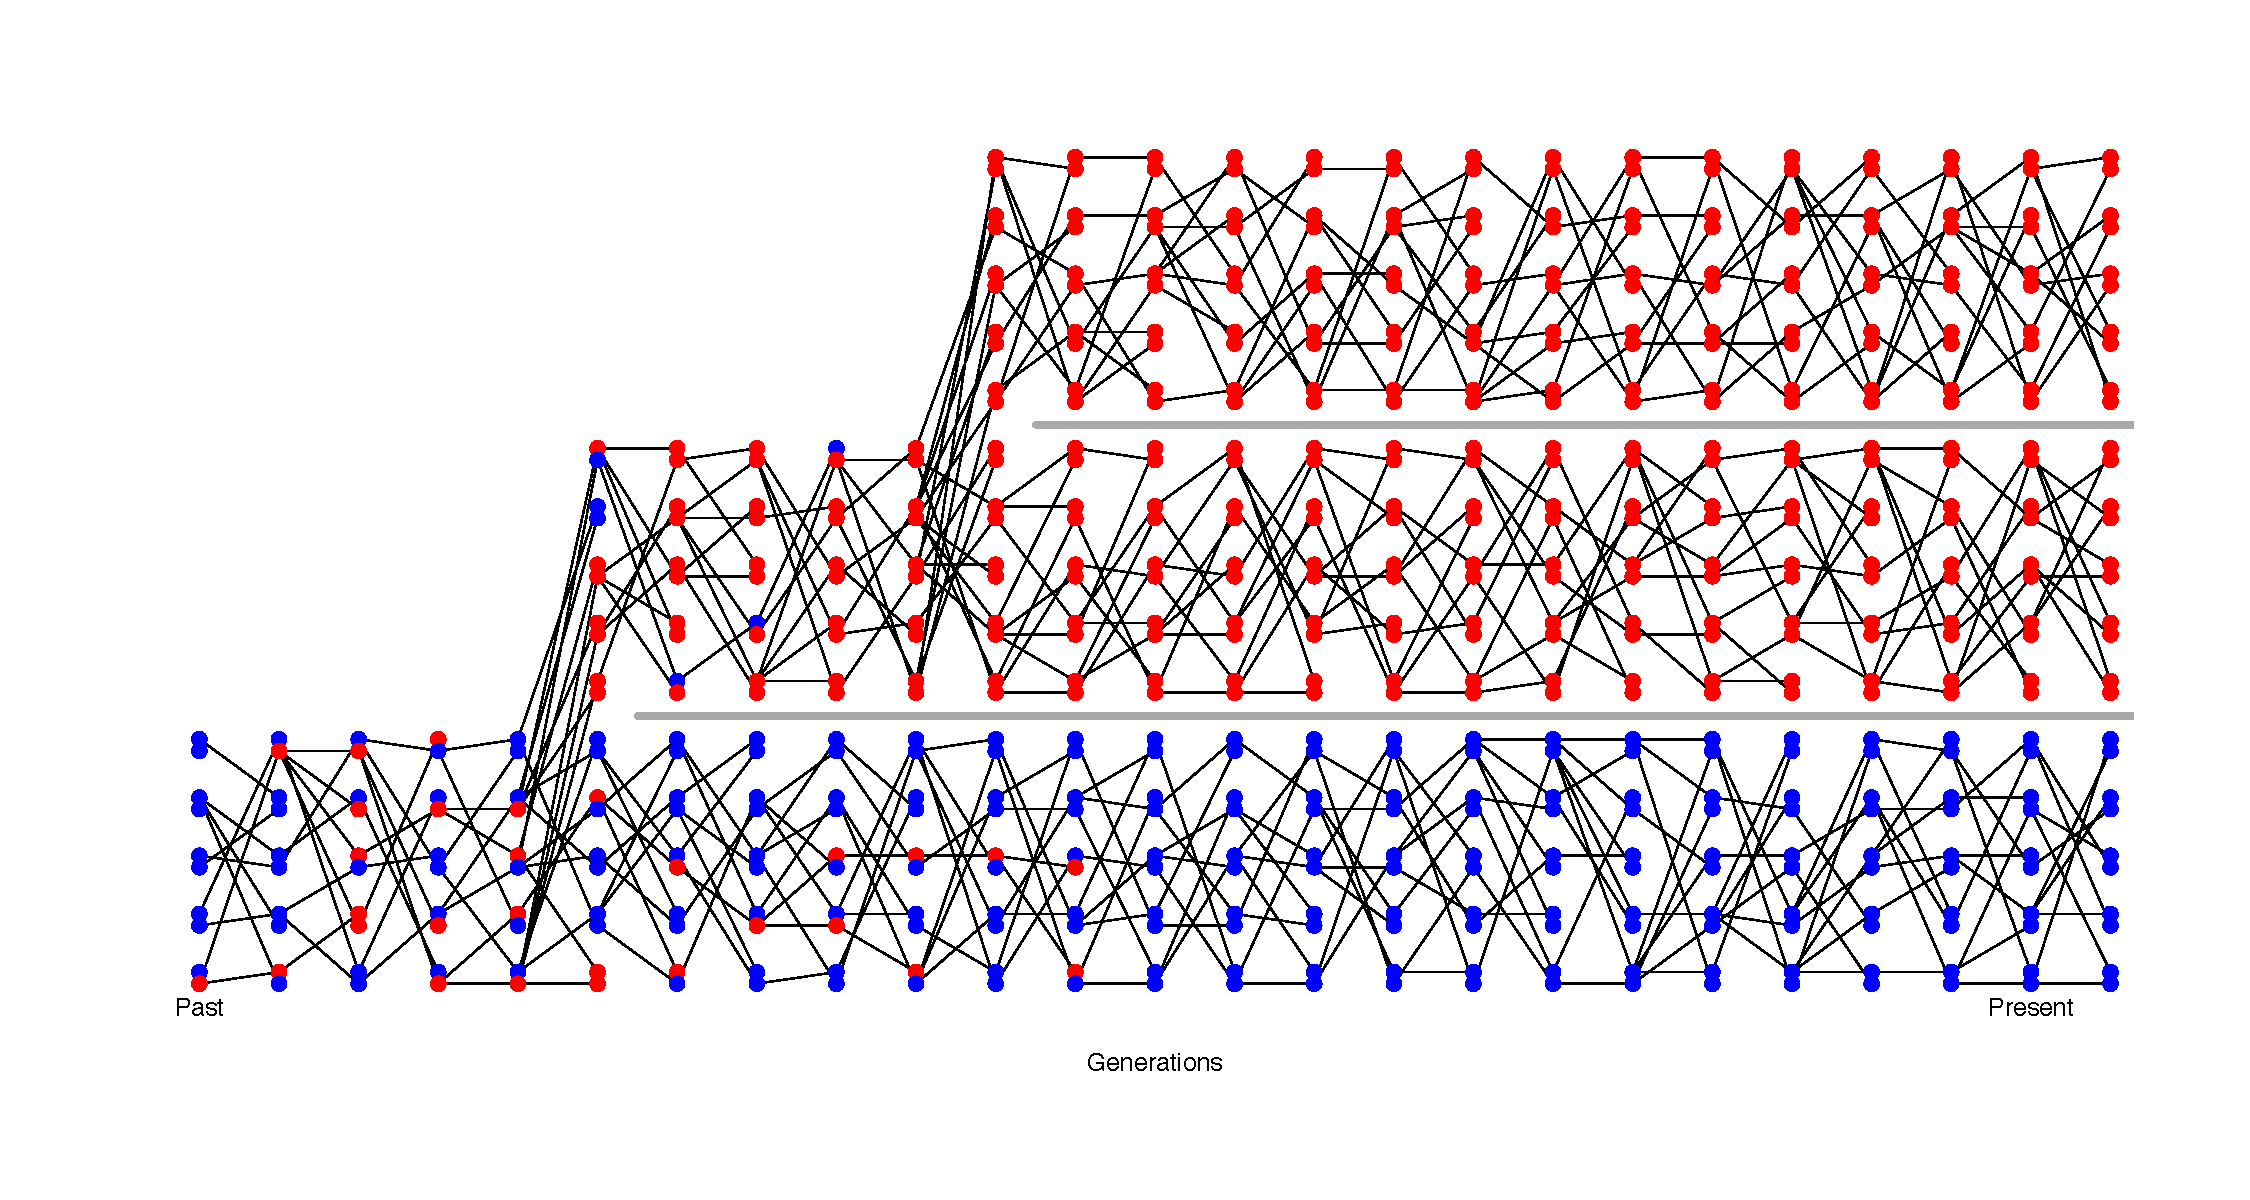
\includegraphics[width=\textwidth]{figures/Genetic_drift/ILS/no_ILS.pdf}
\end{center}
\caption{An example of alleles assorting among three populations such that there is no incomplete lineage sorting. \gitcode{https://github.com/cooplab/popgen-notes/blob/master/Rcode/Loss_of_heterozyg_varying_pop.R}} \label{fig:NoILS_poly}
\end{figure}

\begin{figure}
\begin{center}
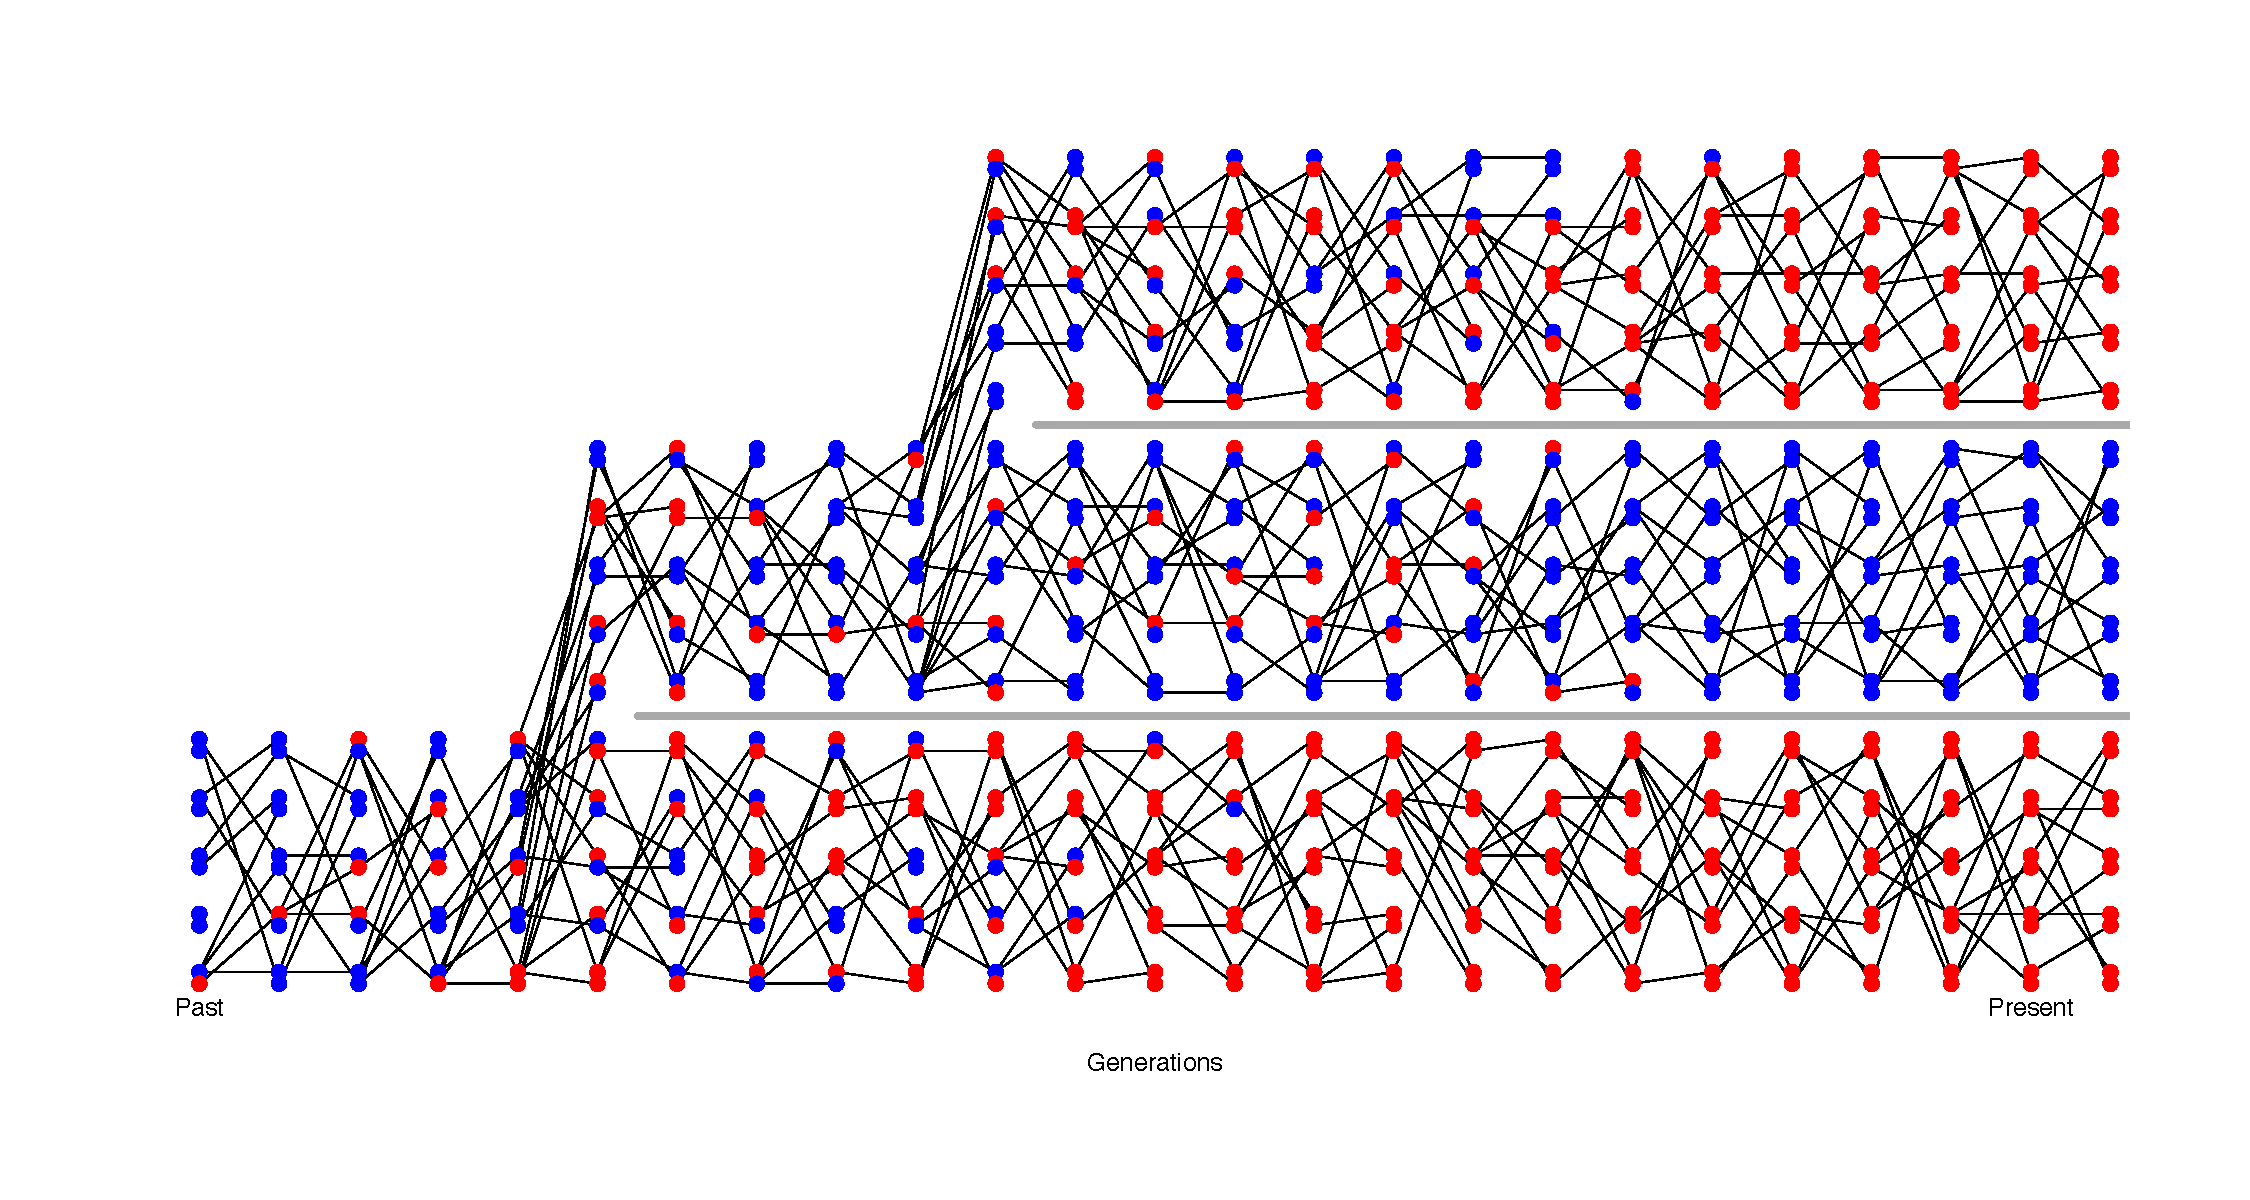
\includegraphics[width=\textwidth]{figures/Genetic_drift/ILS/ILS.pdf}
\end{center}
\caption{An example of alleles assorting among three populations leading to incomplete lineage sorting. \gitcode{https://github.com/cooplab/popgen-notes/blob/master/Rcode/Loss_of_heterozyg_varying_pop.R} } \label{fig:ILS_poly}
\end{figure}


\begin{figure}
\begin{center}
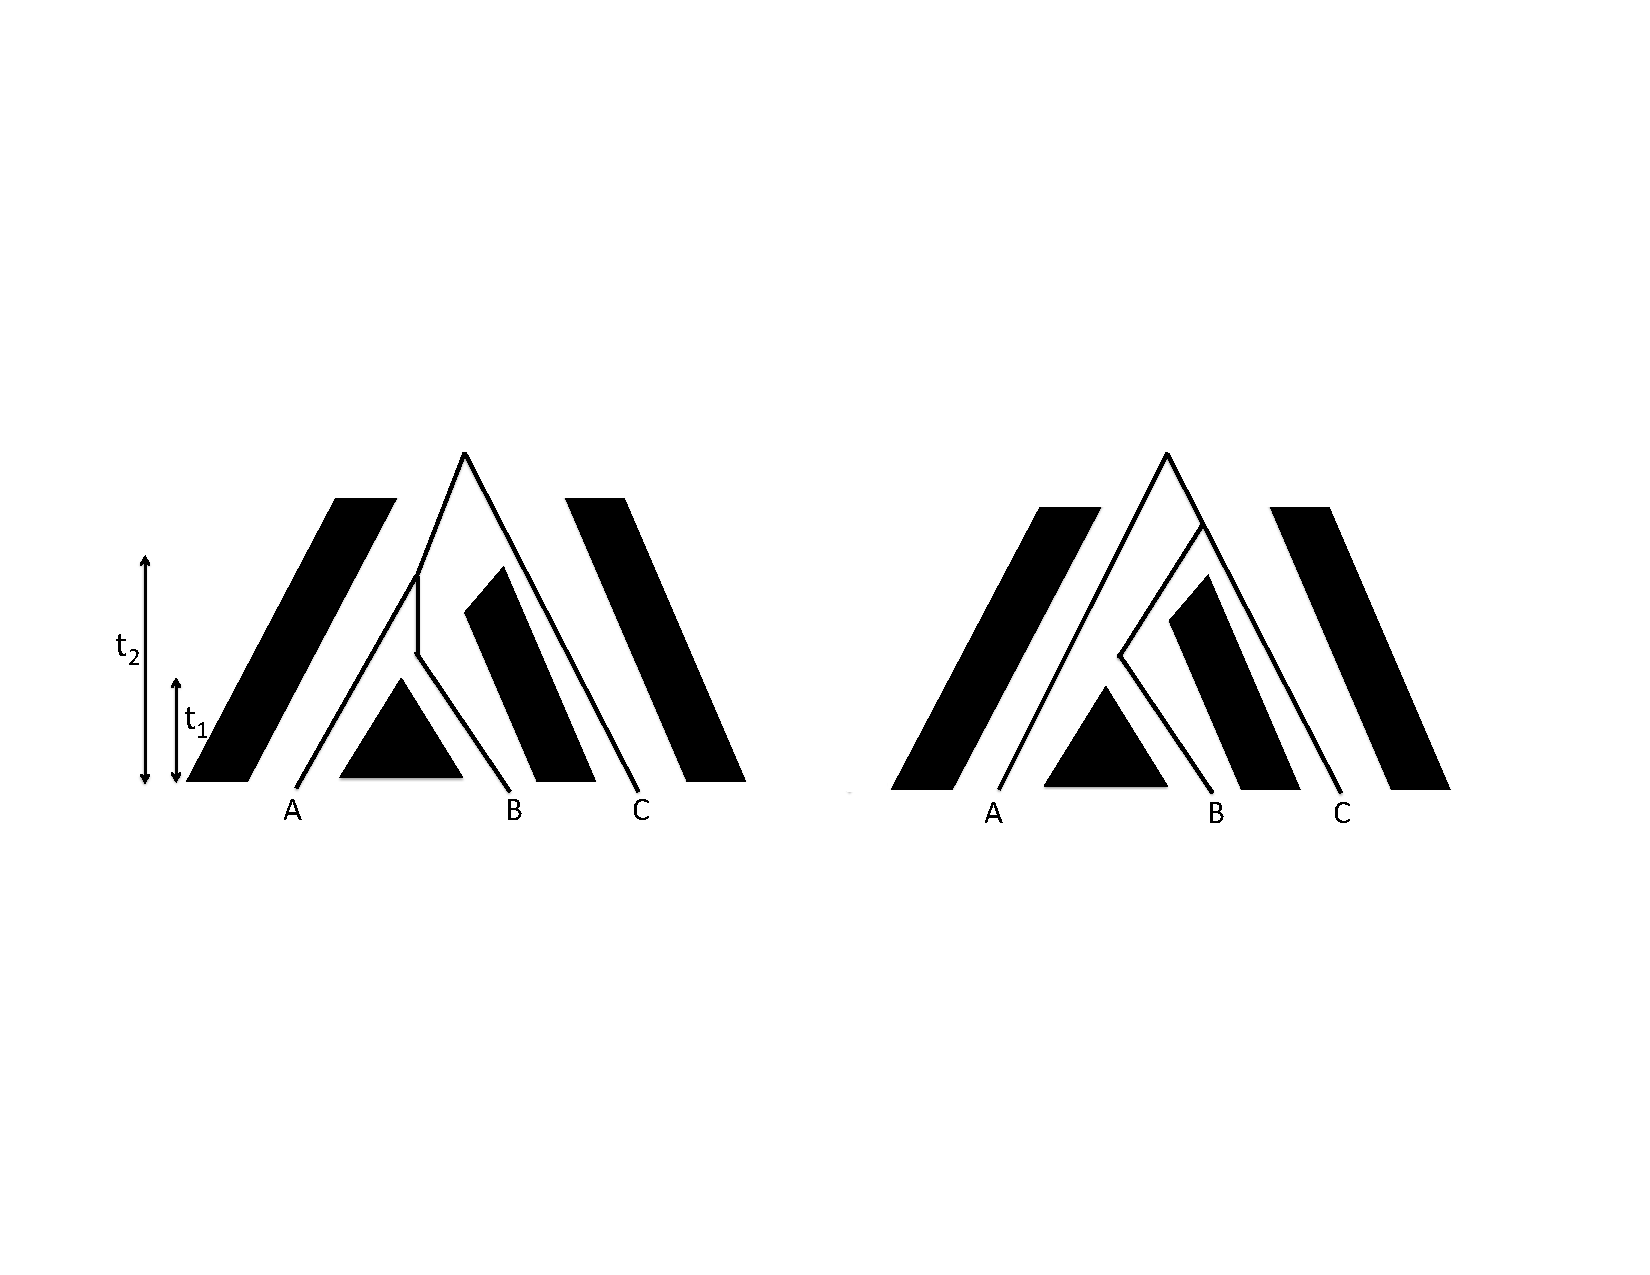
\includegraphics[width=\textwidth]{figures/Genetic_drift/ILS/ILS_coal_cartoon.pdf}
\end{center}
\caption{The population tree of three populations ((A, B), C) is shown
blocked out with black shapes. Two different coalescent trees
relating a single allele drawn from A, B, and C are shown with thinner lines.} \label{fig:ILS_cartoon}
\end{figure}

A natural pedigree analogy to incomplete lineage sorting is the fact that while two
biological siblings are more closely related to each other genealogically than
either is to their cousin, at any given locus one of the siblings can
share an allele IBD with their cousin that they do not share with
their own sibling, due to the randomness of Mendelian segregation down their
pedigree. In these cases, the average relatedness of the individuals/populations disagrees
with the patterns of relatedness at a particular locus.


%\begin{question}
%Draw a pedigree of two full cousins, where one of the cousins has a full sibling. Label the four alleles in shared grandparents 1-4, and draw the situation where the cousins share 1 allele IBD, and the sibs share 0 alleles IBD.
%\end{question}
%This analogy isn't perfect as full cousins dont share one parents, while all three of our populations share one ancestral, parental population far enough back. If we want to make this analogy more perfect we'd need to posit a bunch of inbreeding, but honestly drawinf that would make my head hurt a lot.

\begin{marginfigure}
\begin{center}
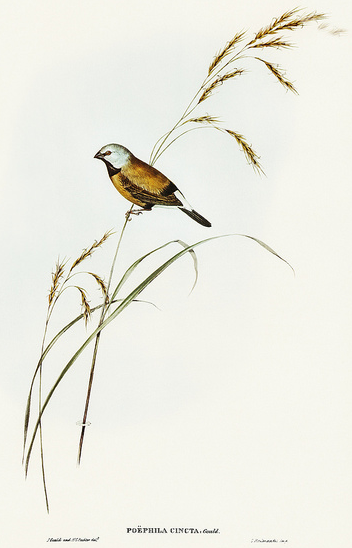
\includegraphics[width=\textwidth]{illustration_images/Genetic_drift/Poephila_cincta_finch/Poephila_cincta_finch.png}
\end{center}
\caption{Banded Grass Finch ({\it P. cincta}). Illustration by
  Elizabeth Gould.
  \newline \noindent \tiny{Birds of Australia Gould J. 1840. CC BY 4.0 uploaded to \href{https://www.flickr.com/photos/vintage_illustration/41073432105/in/photolist-WpHYmR-WBF2Uc-Uoq2kW-QAW9bN-UL33uh-RmyMxt-PKmBjN-8xpKmQ-8xmHg2-H6mfAS-dVREvC-7Qepuh-222xkPQ-7QepzS-25zw6ak-W28Nyk-Qa6d32-ijh2uH-6V8Srd-25zw5ov-8xpKB7-nUQ33T-6V8TLy-nV88oH-25RuYmq-21TcFz1-R2Gdy4-GdWRgi-GdMmry-GdWAwD-9mjwfA-25oHWeJ-HMbQre-6CQWTH-7TjKu-e6SYV-25RuXU3-pdKtxc-9hYCzE-voj7Sj-zqSdQb-6SNmDE-a1datx-a1dasZ-PFfPXY-rR7QYw-GJ7rey-6SJmuB-7TjFh}{Flickr} by \url{rawpixel.com}.}} \label{fig:Poephila_cincta}
\end{marginfigure}

As an empirical example of incomplete lineage sorting, let's consider the work of
\citet{jennings:05} who sequenced a single allele from three
different species of Australian grass finches ({\it Poephila}): two sister species
of long-tailed finches ({\it Poephila acuticauda} and {\it P. hecki})
and the black-throated finch ({\it Poephila cincta}, see Figure \ref{fig:Poephila_cincta}). They collected
sequence data for 30 genes, and constructed phylogenetic gene trees
at each of these loci, resulting in 28 well-resolved gene trees.
16 of the gene trees showed {\it
  P. acuticauda} and {\it P. hecki} as sisters with {\it P. cincta})
(the tree ((A,H),C)~), while for twelve genes the gene tree was
discordant with the population tree: for seven of their genes  {\it P. hecki}
fell as an outgroup to the other two and at five {\it P. acuticauda} fell as an outgroup (the trees ((A,C),H) and
((H,C),A) respectively).


Let's use the coalescent to understand this discordance between gene
trees and species trees. Let's assume that two sister populations
(A \& B) split $t_1$ generations in the past, with a
deeper split from a third outgroup population (C) $t_2$ generations in the
past. We'll assume that there's no gene flow among our populations
after each split. We can trace back the ancestral lineages of our three alleles. The
first opportunity for the A \& B lineages to coalesce is $t_1$
generations ago. If they coalesce with each other in their shared
ancestral population before $t_2$ in the past (left side of
Figure \ref{fig:ILS_cartoon}) their gene tree will
definitely agree with the population tree. So the only way for the gene
tree to disagree with the population tree is for the A \& B lineages
to fail to coalesce in their shared ancestral population between $t_1$ and  $t_2$; this happens
with probability $\left(1 - \nicefrac{1}{2N}\right)^{t_2-t_1}$. We'll
get a discordant gene tree if A
\& B make it back to the shared ancestral population with C without
coalescing, and then one or the other of them coalesces with the C lineage before they coalesce with each other. This happens with probability $2/3$, as at the first
pairwise-coalescent event there are are three possible pairs of lineages that could coalesce, two of
which (A \& C  and B \& C ) result in a discordant tree. So the
probability that we get a coalescent tree that is discordant with the population tree is
\begin{equation}
\frac{2}{3} \left(1 - \nicefrac{1}{2N}\right)^{t_2-t_1}.
\end{equation}
Thus we should expect gene-tree population-tree discordance when populations split in rapid succession and/or population sizes are large.
\begin{question}
Let's return to \citeauthor{jennings:05}'s Australian grass finches
example. They estimated that the ancestral population size of our two
long-tailed finches was four hundred thousand. What is your best
estimate of the inter-speciation time, i.e. $t_2-t_1$?
\end{question}

\paragraph{Testing for gene flow.}

We often want to test whether gene flow has occurred between populations. For example, we might want to establish a case
that interbreeding between humans and Neanderthals occurred or demonstrate that
gene flow occurred after two populations began to speciate.
A broad range of methods have been designed to test for gene flow and
to estimate gene flow rates based on neutral expectations. Here we'll briefly just discuss one method based on
some simple coalescent ideas.  Above we assumed that gene-tree population-tree discordance was due to
incomplete lineage sorting due to populations rapidly
splitting. However, gene flow among populations can also lead to gene-tree discordance.
While both ILS and gene flow can lead to discordance, under
simplifying assumptions, ILS implies more symmetry in how these
discordances manifest themselves.\\


\begin{figure}
\begin{center}
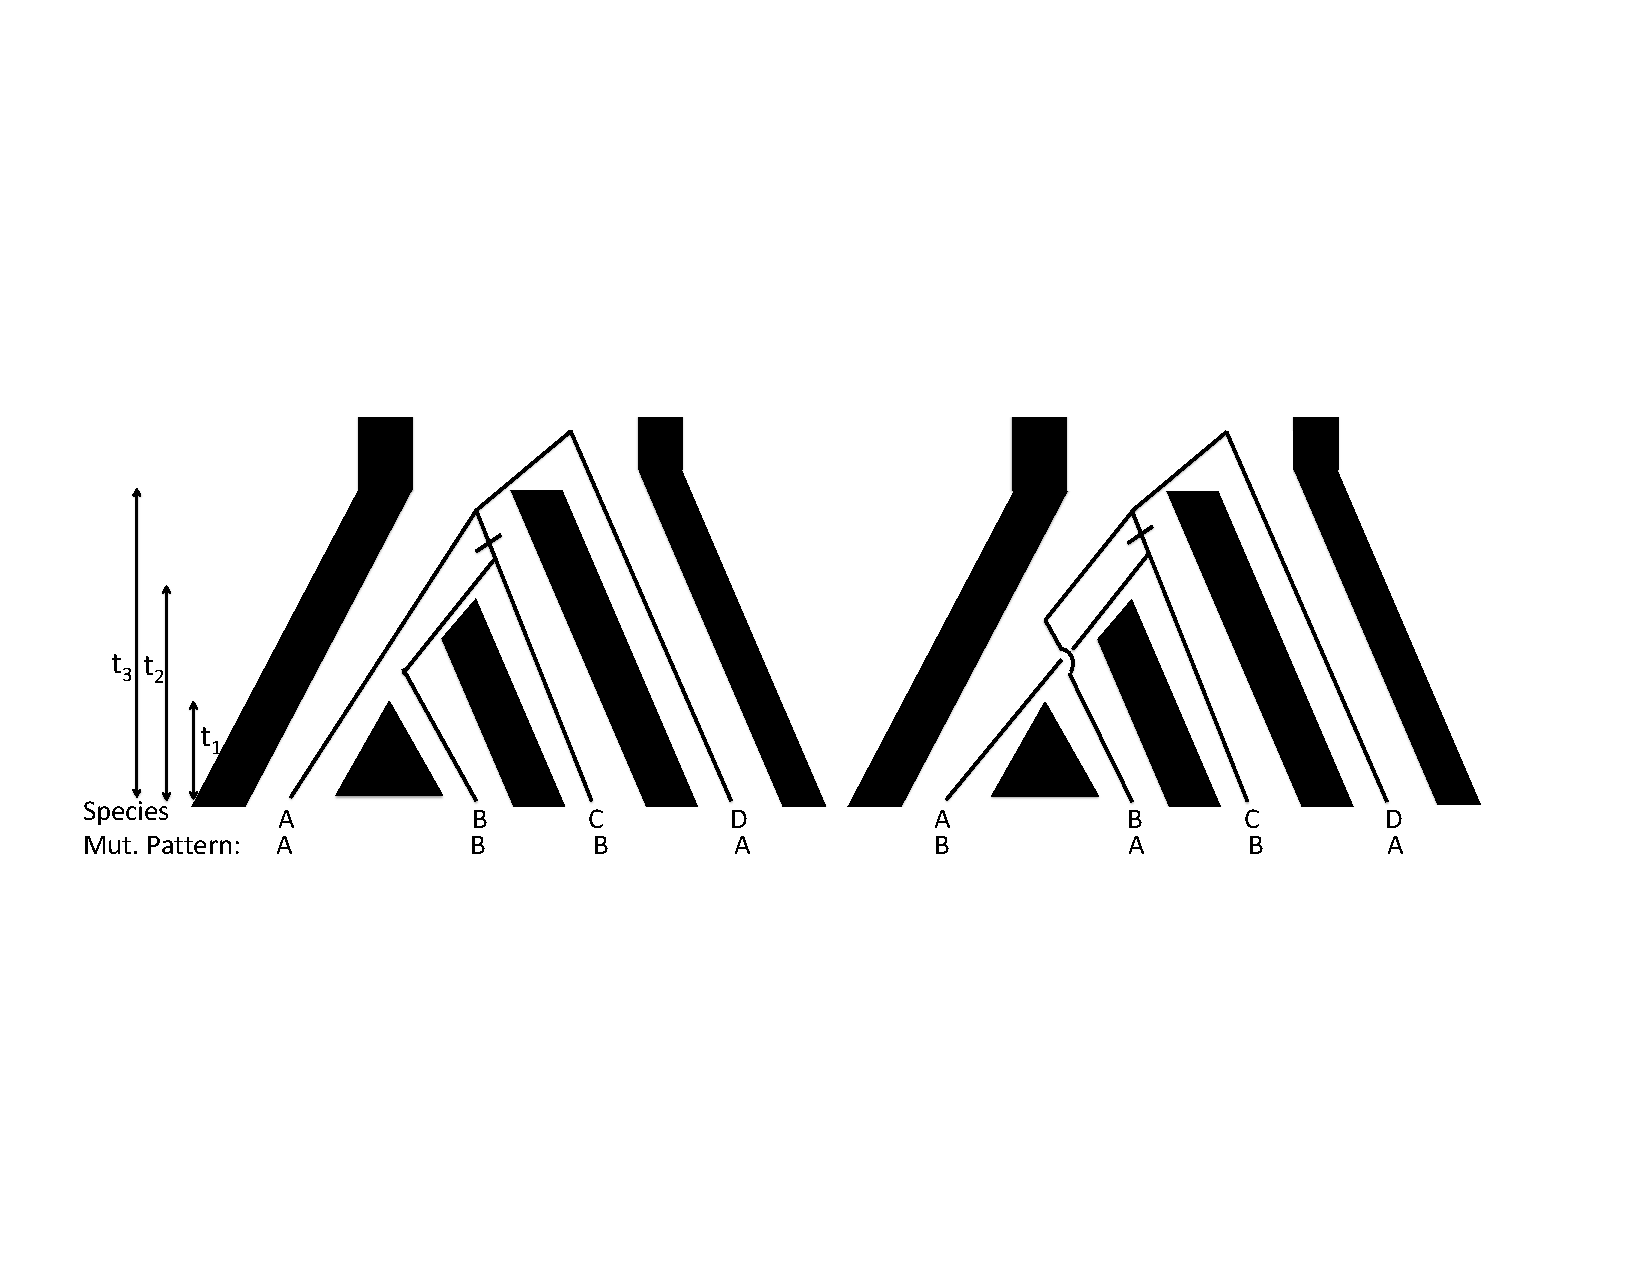
\includegraphics[width=\textwidth]{figures/Genetic_drift/ILS/ABBA_BABA_coal.pdf}
\end{center}
\caption{ In both the left and and right trees ILS has occurred between our single lineages sampled from populations A, B, and C. Imagine that population D is a somewhat distant outgroup
such that the lineages from A through C (nearly) always coalesce with each other before any coalesce with D. The small dash on the branch indicates the mutation A$\rightarrow$B occurring, giving rise to the
ABBA or BABA mutational pattern shown at the bottom. } \label{fig:ABBA_BABA}
\end{figure}
%JRI: here and in text you refer to populations ABCD but figure is labelled ``species'' and 1234. I think ABCD for populations and AB for alleles is confusing. I don't know if you need A/B for alleles. Why not use A1A2 or just 1/2 as you have previously? sure you miss the fun mnemonic, but it's clearer for a novice reader

Take a look at Figure \ref{fig:ABBA_BABA}. In both cases the lineages from A and B fail to coalesce in
their initial shared ancestral population, and one or the other of them
coalesces with the lineage from C before they coalesce with each other. Each option is equally
likely; therefore the mutational patterns ABBA and BABA are equally likely to occur under ILS.  \sidenote{Here we have to assume no structure in the ancestral population.}

However, if gene flow occurs from population C into population B, in addition to ILS the lineage from B can more recently coalesce with the lineage from C, and so we should see more ABBAs than BABAs. To test for this effect of gene flow, we can sample a sequence from each of our 4 populations and count up the number of sites that show the two mutational patterns consistent with the gene-tree discordance $n_{ABBA}$ and
$n_{BABA}$ and calculate
\begin{equation}
\frac{n_{ABBA}-n_{BABA}}{n_{ABBA}+n_{BABA}}
\end{equation}
This statistic will have expectation zero if the gene-tree discordance is due to ILS and will be skewed negative if gene flow
occurred from C into B (and skewed positive if gene flow occurred from C into A).
\graham{Add ABABA BABA egs}
